\section{Regret Analysis}
\label{sec:RegretAnalysis}

Recall from \autoref{ch:LiteratureReview} that the cumulative regret of the UCB1 algorithm is proportional to log($n$), where $n$ is the number of plays. Thus, we should expect the UCB1-AKSB algorithm to result in a cumulative pseudo-regret that is approximately logarithmic in the number of plays. This empirical pseudo-regret, $\hat{R}_n$, was calculated using \autoref{eq:RegretComputation} below under the assumptions that the long-term average de-anonymization proportion was optimal.

\begin{equation}
\label{eq:RegretComputation}
\hat{R}_n = \mu^{*}n - \sum_{t=1}^{n}{X_{I_t, t}}
\end{equation}

In \autoref{eq:RegretComputation}, $\mu^{*}n$ is the expected optimal number of de-anonymizations by play $n$ (i.e. $\max_{i=1,...,K}{\mathbb{E}\left[\sum_{t=1}^{n}{X_{i, t}}\right]}$ from \autoref{eq:PseudoRegret}). The plot of $\hat{R}_n$ as a function of $n$ for the UCB1-AKSB algorithm is shown below in \autoref{fig:TADe-AnonymizationRegret}.

\begin{figure}[H]
\centering
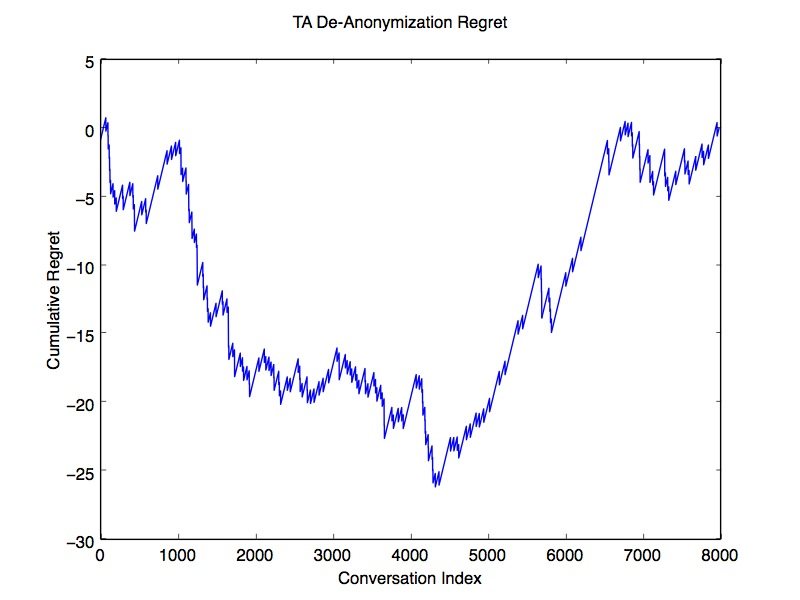
\includegraphics[trim= 0mm 0mm 0mm 0mm, clip, scale=0.5]{./Figures/TADe-AnonymizationRegret.jpg}
\caption{TA De-Anonymization Regret Analysis}
\label{fig:TADe-AnonymizationRegret}
\end{figure}

The regret looks approximately logarithmic for the second half of the dataset, but the first half of the data gives a steadily negative cumulative regret. This is due to the fact that the I.I.D assumption of conversation de-anonymization is most-likely false. Instead, there were probably different regimes in which people perceived Facebook de-anonymization differently. This is most analogous to the Markovian bandits in \cite{bubeck12}, where each conversation starter (i.e. bandit arm) is associated with a Markov process with a discrete set of distributions.

Because of the clear split in the data, it seems like there were two discrete distributions from which de-anonymizations were drawn. The first distribution occurred in the initial stages of TA's launch, where users were more likely to de-anonymize a conversation simply because of the novelty of doing so. This is supported by looking at the initial cumulative Facebook de-anonymization statistics (see \autoref{fig:TADe-AnonymizationCumulative}), where the Facebook connect rate was almost double the long-term average. The second distribution most likely occurred as users became more used to the idea of anonymity (and probably began to enjoy it), thus resulting in a lower conversation de-anonymization rate. The existence of multiple regimes explains the two parts of the regret data in \autoref{fig:TADe-AnonymizationRegret}.

\begin{figure}[H]
\centering
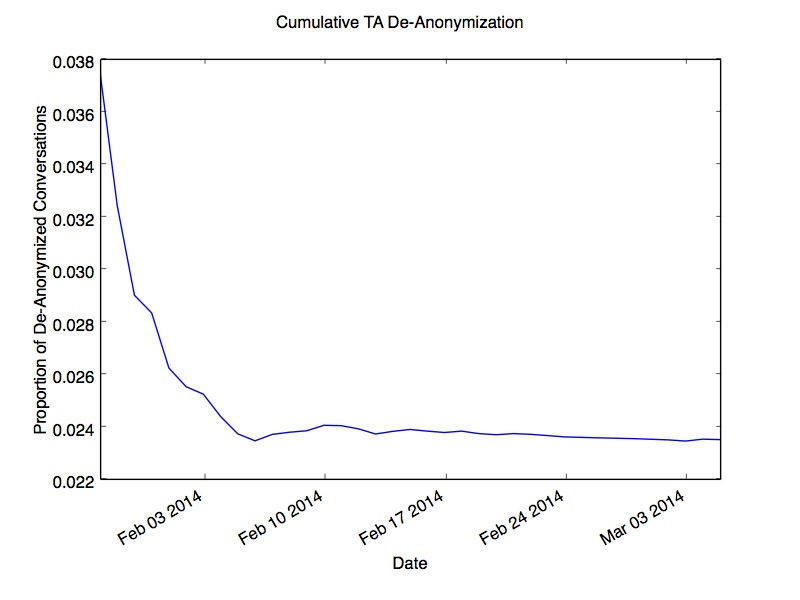
\includegraphics[trim= 0mm 0mm 0mm 0mm, clip, scale=0.5]{./Figures/CumulativeTADe-Anonymization.jpg}
\caption{TA Cumulative Conversation De-Anonymization Rate}
\label{fig:TADe-AnonymizationCumulative}
\end{figure}

\section{UCB1-AKSB Effectiveness}

Since conversation de-anonymization was the metric that UCB1-AKSB used to judge each bandit arm, the obvious way to measure the performance of the UCB1-AKSB algorithm is the proportion of conversations which were de-anonymized. Judging from not only the cumulative de-anonymization proportion (\autoref{fig:TADe-AnonymizationCumulative}), but also the daily de-anonymization proportion (\autoref{fig:TADe-AnonymizationDaily}), it seems that the algorithm had little impact on whether or not people opted to de-anonymize the conversation. If anything, it looks like the algorithm had an adverse impact on conversation de-anonymization.

However, this may have been due to the fact that the user's decision to de-anonymize the conversation was based on factors other than the conversation starter. It is easy to imagine a case in which the conversation was extremely revealing and thus users were hesitant to reveal their identities for fear of being connected to the conversation. In such cases, the conversation starter may have been excellent (and would have led to de-anonymization in some cases), but in other cases, the tendencies of the specific users would prevent them from de-anonymizing after the conversation had progressed past a certain level. In other words, the process of conversation de-anonymization might have been more user-specific (i.e. context dependent) than the UCB1-AKSB algorithm assumed, which could have resulted in a downward drag on de-anonymization rates even as the conversation starter quality improved.

Another possible explanation for falling de-anonymization rates is the increasing fascination with anonymity as mentioned in the previous section: over time, TA's perception changed from a site to make new connections to a site to have anonymous conversations, with user behavior adjusting accordingly. This is also consistent with the multiple regimes that can be seen in the cumulative psuedo-regret data in the previous section.

Finally, even if the process of conversation de-anonymization was sufficiently user-independent for the UCB1-AKSB algorithm to work properly, the metric itself is not granular to accurately measure incremental improvements. For example, let's say the conversation de-anonymization would only occur if the conversation `quality' metric was above some threshold $d$. Even if the UCB1-AKSB algorithm boosted the quality of otherwise low-quality conversation by providing some common ground, such a quality boost would not be visible unless the incremental improvement was enough to make such conversations pass the threshold $d$. Basically, it is entirely possible that the UCB1-AKSB algorithm could improve conversation quality but this increased likelihood would not be visible because of the censored data observed. This censored-data hypothesis would also explain some of the erratic behavior of the daily de-anonymization rate seen in \autoref{fig:TADe-AnonymizationDaily}.

\begin{figure}[H]
\centering
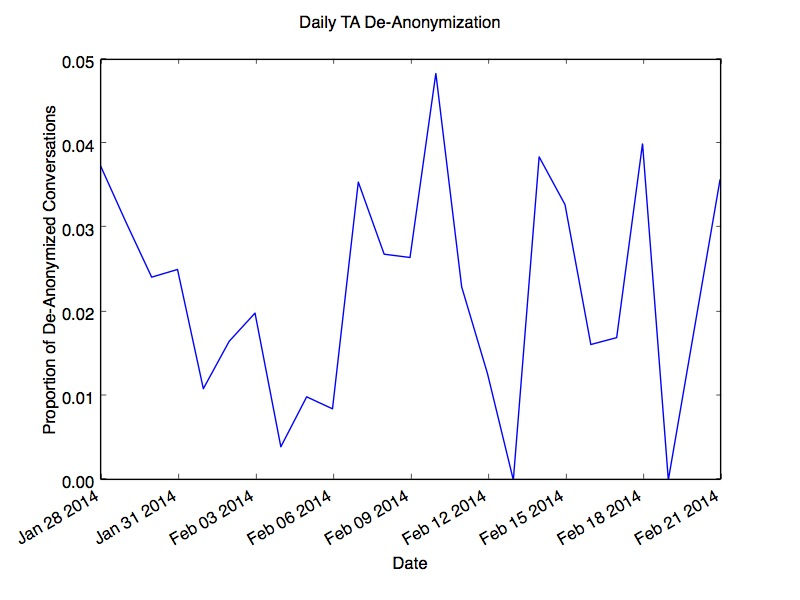
\includegraphics[trim= 0mm 0mm 0mm 0mm, clip, scale=0.5]{./Figures/DailyTADe-Anonymization.jpg}
\caption{TA Daily Conversation De-Anonymization Rate}
\label{fig:TADe-AnonymizationDaily}
\end{figure}

Given that conversation de-anonymization might have been affected by other exogenous variables and was not granular enough to measure incremental improvements in conversation quality, it makes sense to turn to other conversation quality metrics to judge the performance of UCB1-AKSB. These other metrics (participation rates and average conversation rates) are less likely to be influenced by the social pressure for or against de-anonymization, as well as having a more finely differentiated set of values than the binary variable of conversation de-anonymization. The plots of both these metrics are shown below in \autoref{fig:TAParticipationCumulative} and \autoref{fig:TAMessagesExchangedCumulative}.

\begin{figure}[H]
\centering
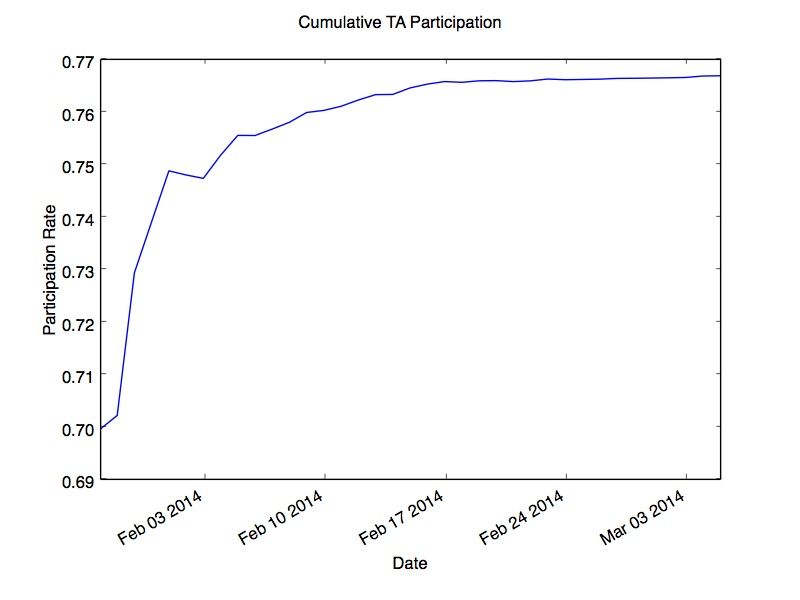
\includegraphics[trim= 0mm 0mm 0mm 0mm, clip, scale=0.5]{./Figures/CumulativeTAParticipation.jpg}
\caption{TA Cumulative Participation Rate}
\label{fig:TAParticipationCumulative}
\end{figure}

\begin{figure}[H]
\centering
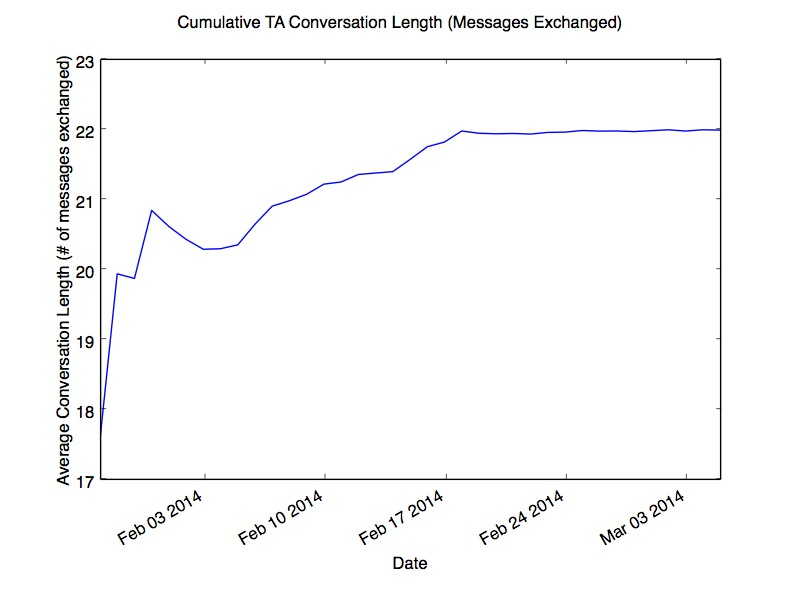
\includegraphics[trim= 0mm 0mm 0mm 0mm, clip, scale=0.5]{./Figures/CumulativeTAConversationLength(MessagesExchanged).jpg}
\caption{TA Cumulative Average Conversation Length}
\label{fig:TAMessagesExchangedCumulative}
\end{figure}

By these metrics, it seems that conversation quality improved noticeably over the course of the user experience, which suggests that the UCB1-AKSB algorithm may still have had a positive effect on conversation quality even though some of its fundamental assumptions weren't true.

\section{Individual User Analysis}
\label{sec:IndividualUserAnalysis}

Another way of examining the data is to look at how individual users as they continued to interact with the site. In each of the plots below, the x-axis represents the number of uses, while the y-axis represents the conditional mean of the metric over the set of users on the $n$-th use, given that they've used the site greater than or equal to n times. In order to define this more clearly, I introduce the following notation: let $f_k(u, n)$ give the value of conversational quality metric $k$ for user $u$ on their $n$-th visit and function $g(u)$ give the number of times user $u$ has visited the site. Let $U_n$ be the set $\{u | u \in {U}, g(u) \geq{n}\}$ (i.e. the set of users who have visited the site at least $n$ times). Then, the graphs below are plots of the following functions $y_k(n)$ for different conversational quality metrics $k$.

$$ y_k(n) = \frac{1}{|U_n|}\sum_{u \in U_n}{f_k(u, n)} $$

\begin{figure}[H]
\centering
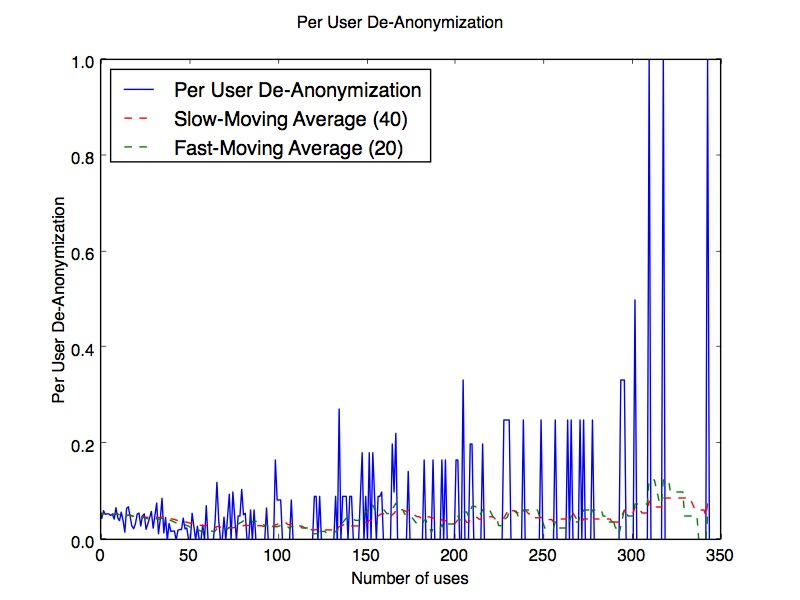
\includegraphics[trim= 0mm 0mm 0mm 0mm, clip, scale=0.5]{./Figures/PerUserDe-Anonymization.jpg}
\caption{De-Anonymization Rate Per User}
\label{fig:PerUserFBConnect}
\end{figure}

\begin{figure}[H]
\centering
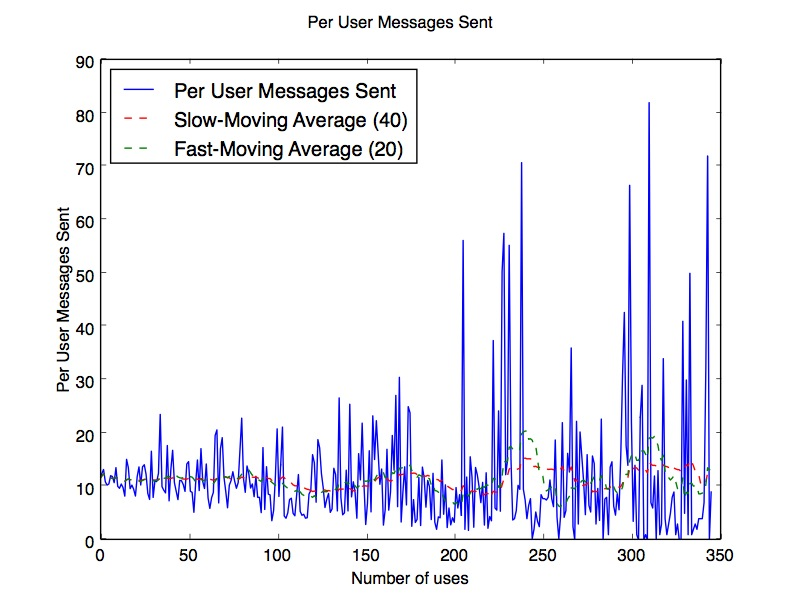
\includegraphics[trim= 0mm 0mm 0mm 0mm, clip, scale=0.5]{./Figures/PerUserMessagesSent.jpg}
\caption{Total Messages Sent Per User}
\label{fig:PerUserMessagesSent}
\end{figure}

\begin{figure}[H]
\centering
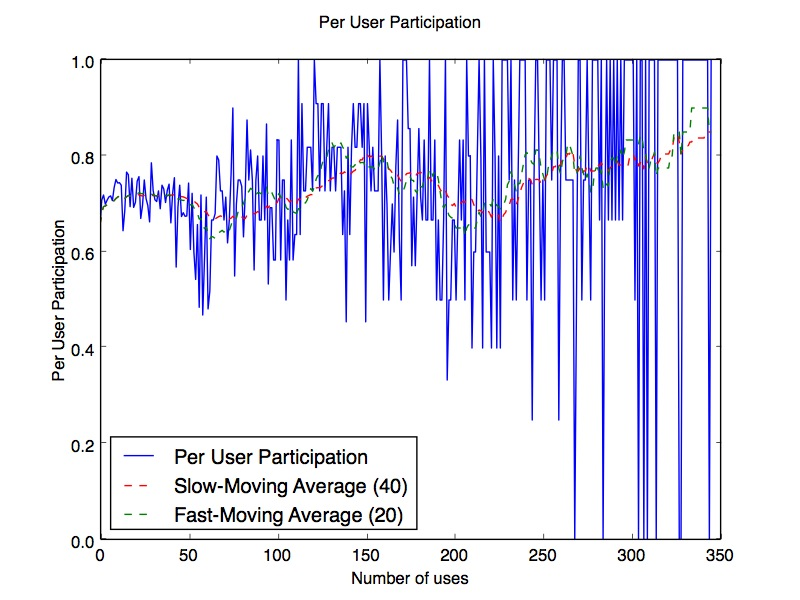
\includegraphics[trim= 0mm 0mm 0mm 0mm, clip, scale=0.5]{./Figures/PerUserParticipation.jpg}
\caption{Participation Rate Per User}
\label{fig:PerUserParticipation}
\end{figure}

The two things that immediately stand out about these plots are the general upward drift over time and increasing volatility over time. The general upward drift of each conversation quality metric on a user-level supports the hypothesis that the UCB1-AKSB was increasing conversation quality over time. Another possible source of this upward drift is that users who visit the site frequently (who I will refer to as power-users) are more interested in having high-quality conversations and will seek to do so independently of the conversation starter. However, even if the latter hypothesis is true, the UCB1-AKSB algorithm still succeeded in providing a set of initial conversation starters to these users to make them want to become power-users, so there is still evidence that the UCB1-AKSB algorithm was effective. Additionally, the steady increase in conversation de-anonymization rate (\autoref{PerUserFBConnect}) suggests that the algorithm actually performed quite well on a per-user basis, even though the cumulative de-anonymization performance was relatively poor (\autoref{TADe-AnonymizationCumulative}).

On the other hand, the increasing volatility over time of each conversation quality metric represents the stratification of users into different classes. An abrupt change from a participation rate of 1.0 to 0.0 in one use is most likely the result of a power-user being paired with an first-time user, so that the first-time user disconnects from the conversation before the power-user has a chance to participate at all.

This stratification of users into extremely high and extremely low involvement raises the issue of user saturation: people were either hooked and used the site extremely frequently or they used it a few times and then left. As a result, the site became saturated with a small fraction of hard-core users, and a large segment of users visited the site infrequently at best. This would result in poor user experience for both classes of users: the new users still have't gotten used to the idea of an anonymous conversation and might be intimidated by a conversation with a power-user, but bored with a conversation with another new-user. Conversely, a power-user would be used to the concept of an anonymous conversation and would be interested in a real conversation: they would most likely get bored with the small-talk of a new user (who still is operating in normal conversation mode) but would quickly run out of new power users to talk to. 

The solution to this problem is to have a `casual user': one who can bridge the gap between the two previous user categories and provide a better TA experience for all. However, the problem that TA ran into with Princeton is the size of the potential user base: people at Princeton who would rather use TA over socializing with their current friends. This user base is not very large, but what if it were possible to combine such a user base from multiple schools into an even larger user base? This is the motivation for the project that I'm currently working on: a larger version of Tigers Anonymous called Campus Anonymous, which will be released to all the universities in the Ivy League, thus broadening the user base and increasing the likelihood of attracting a non-trivial set of `casual users'.
